\begin{frame}{A Map of Prompt Compression}
  \begin{columns}[T,onlytextwidth]
    \column{0.46\textwidth}
      \begin{itemize}\scriptsize\itemsep0.45em
        \item[\textcolor{red}{$\blacktriangleright$}] Prompt compression shortens the input itself: fewer tokens, or a few vectors in place of many tokens. The model then runs as usual on the shorter input, so it stacks with the other techniques.
        \item[\textcolor{red}{$\blacktriangleright$}] The \textbf{compression ratio} is $n/\tilde n$, where $n$ is the number of tokens in the original prompt and $\tilde n$ the number of tokens or vectors the LLM reads instead. LLMLingua cuts a 2,366-token prompt to 117 tokens (next slide), a ratio of about $20\times$.
        \item[\textcolor{red}{$\blacktriangleright$}] \textbf{Hard} methods output text: here a subset of the original tokens, though paraphrasing methods also count as hard. A \textbf{black-box} model, reachable only through a text API, can read it, and a person can audit it.
        \item[\textcolor{red}{$\blacktriangleright$}] \textbf{Soft} methods output vectors the LLM reads in place of tokens, as input embeddings or as keys and values at every layer. They need the weights and some training.
        \item[\textcolor{red}{$\blacktriangleright$}] \textbf{Query-aware} methods see the question and keep what it needs; \textbf{query-agnostic} methods compress once and reuse the result for any question.
      \end{itemize}
    \column{0.52\textwidth}
      \centering
      \vspace{0.2em}
      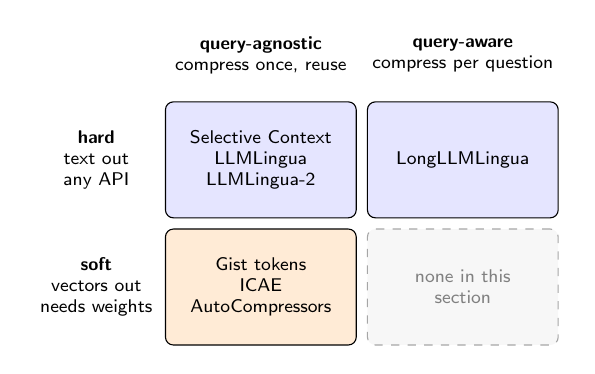
\begin{tikzpicture}[font=\sffamily\scriptsize, scale=0.95,
          every node/.style={transform shape},
          cell/.style={draw, rounded corners=0.1cm, align=center, minimum width=2.55cm, minimum height=1.55cm},
          hardcell/.style={cell, fill=blue!10},
          softcell/.style={cell, fill=orange!16},
          emptycell/.style={cell, dashed, draw=gray!70, fill=gray!6, text=gray},
          head/.style={align=center, text width=2.55cm},
          rowhead/.style={align=center, text width=1.6cm}]
        \node[head] at (2.95,3.25) {\textbf{query-agnostic}\\compress once, reuse};
        \node[head] at (5.65,3.25) {\textbf{query-aware}\\compress per question};
        \node[rowhead] at (0.75,1.85) {\textbf{hard}\\text out\\any API};
        \node[rowhead] at (0.75,0.15) {\textbf{soft}\\vectors out\\needs weights};
        \node[hardcell] at (2.95,1.85) {Selective Context\\LLMLingua\\LLMLingua-2};
        \node[hardcell] at (5.65,1.85) {LongLLMLingua};
        \node[softcell] at (2.95,0.15) {Gist tokens\\ICAE\\AutoCompressors};
        \node[emptycell] at (5.65,0.15) {none in this\\section};
      \end{tikzpicture}\\[0.4em]
      {\scriptsize Two independent choices: what the compressor outputs, and whether it sees the question. Every soft method here compresses without the question, so its vectors can be computed once and cached.\par}
      \vspace{0.3em}
      {\scriptsize Hard/soft split after Li et al., ``Prompt Compression for Large Language Models: A Survey,'' NAACL 2025, \href{https://aclanthology.org/2025.naacl-long.368/}{aclanthology.org/2025.naacl-long.368}.\par}
  \end{columns}
\end{frame}

\begin{frame}{Deleting Low-Information Tokens}
  \begin{columns}[T,onlytextwidth]
    \column{0.46\textwidth}
      \begin{itemize}\scriptsize\itemsep0.35em
        \item[\textcolor{red}{$\blacktriangleright$}] \textbf{Selective Context} scores each token with a small causal LM by its \textbf{self-information}
          \[ I(x_t) = -\log_2 p(x_t \mid x_{<t}), \]
          where $x_t$ is the $t$-th prompt token and $p$ the small model's next-token probability. Predictable tokens carry little information. Perplexity is 2 raised to the mean of $I$.
        \item[\textcolor{red}{$\blacktriangleright$}] Token scores are summed over noun phrases (self-information is additive) and phrases below a chosen percentile are deleted. Deleting half cut per-token time from 110.8 to 76.3\,ms in the paper's Vicuna-13B example. Averaged over all models, BERTScore, an embedding similarity to the full-context answer, fell by 0.023.
        \item[\textcolor{red}{$\blacktriangleright$}] \textbf{LLMLingua} adds three parts. A \textbf{budget controller} keeps 85\% of the instruction and 90\% of the question, and drops whole demonstrations first, lowest perplexity first. \textbf{Iterative token-level compression} scores 100-token segments given the text already compressed, because a deletion changes how surprising the next token is. \textbf{Distribution alignment} instruction-tunes the small LM on text generated by the target LLM.
      \end{itemize}
    \column{0.52\textwidth}
      \centering
      \vspace{0.4em}
      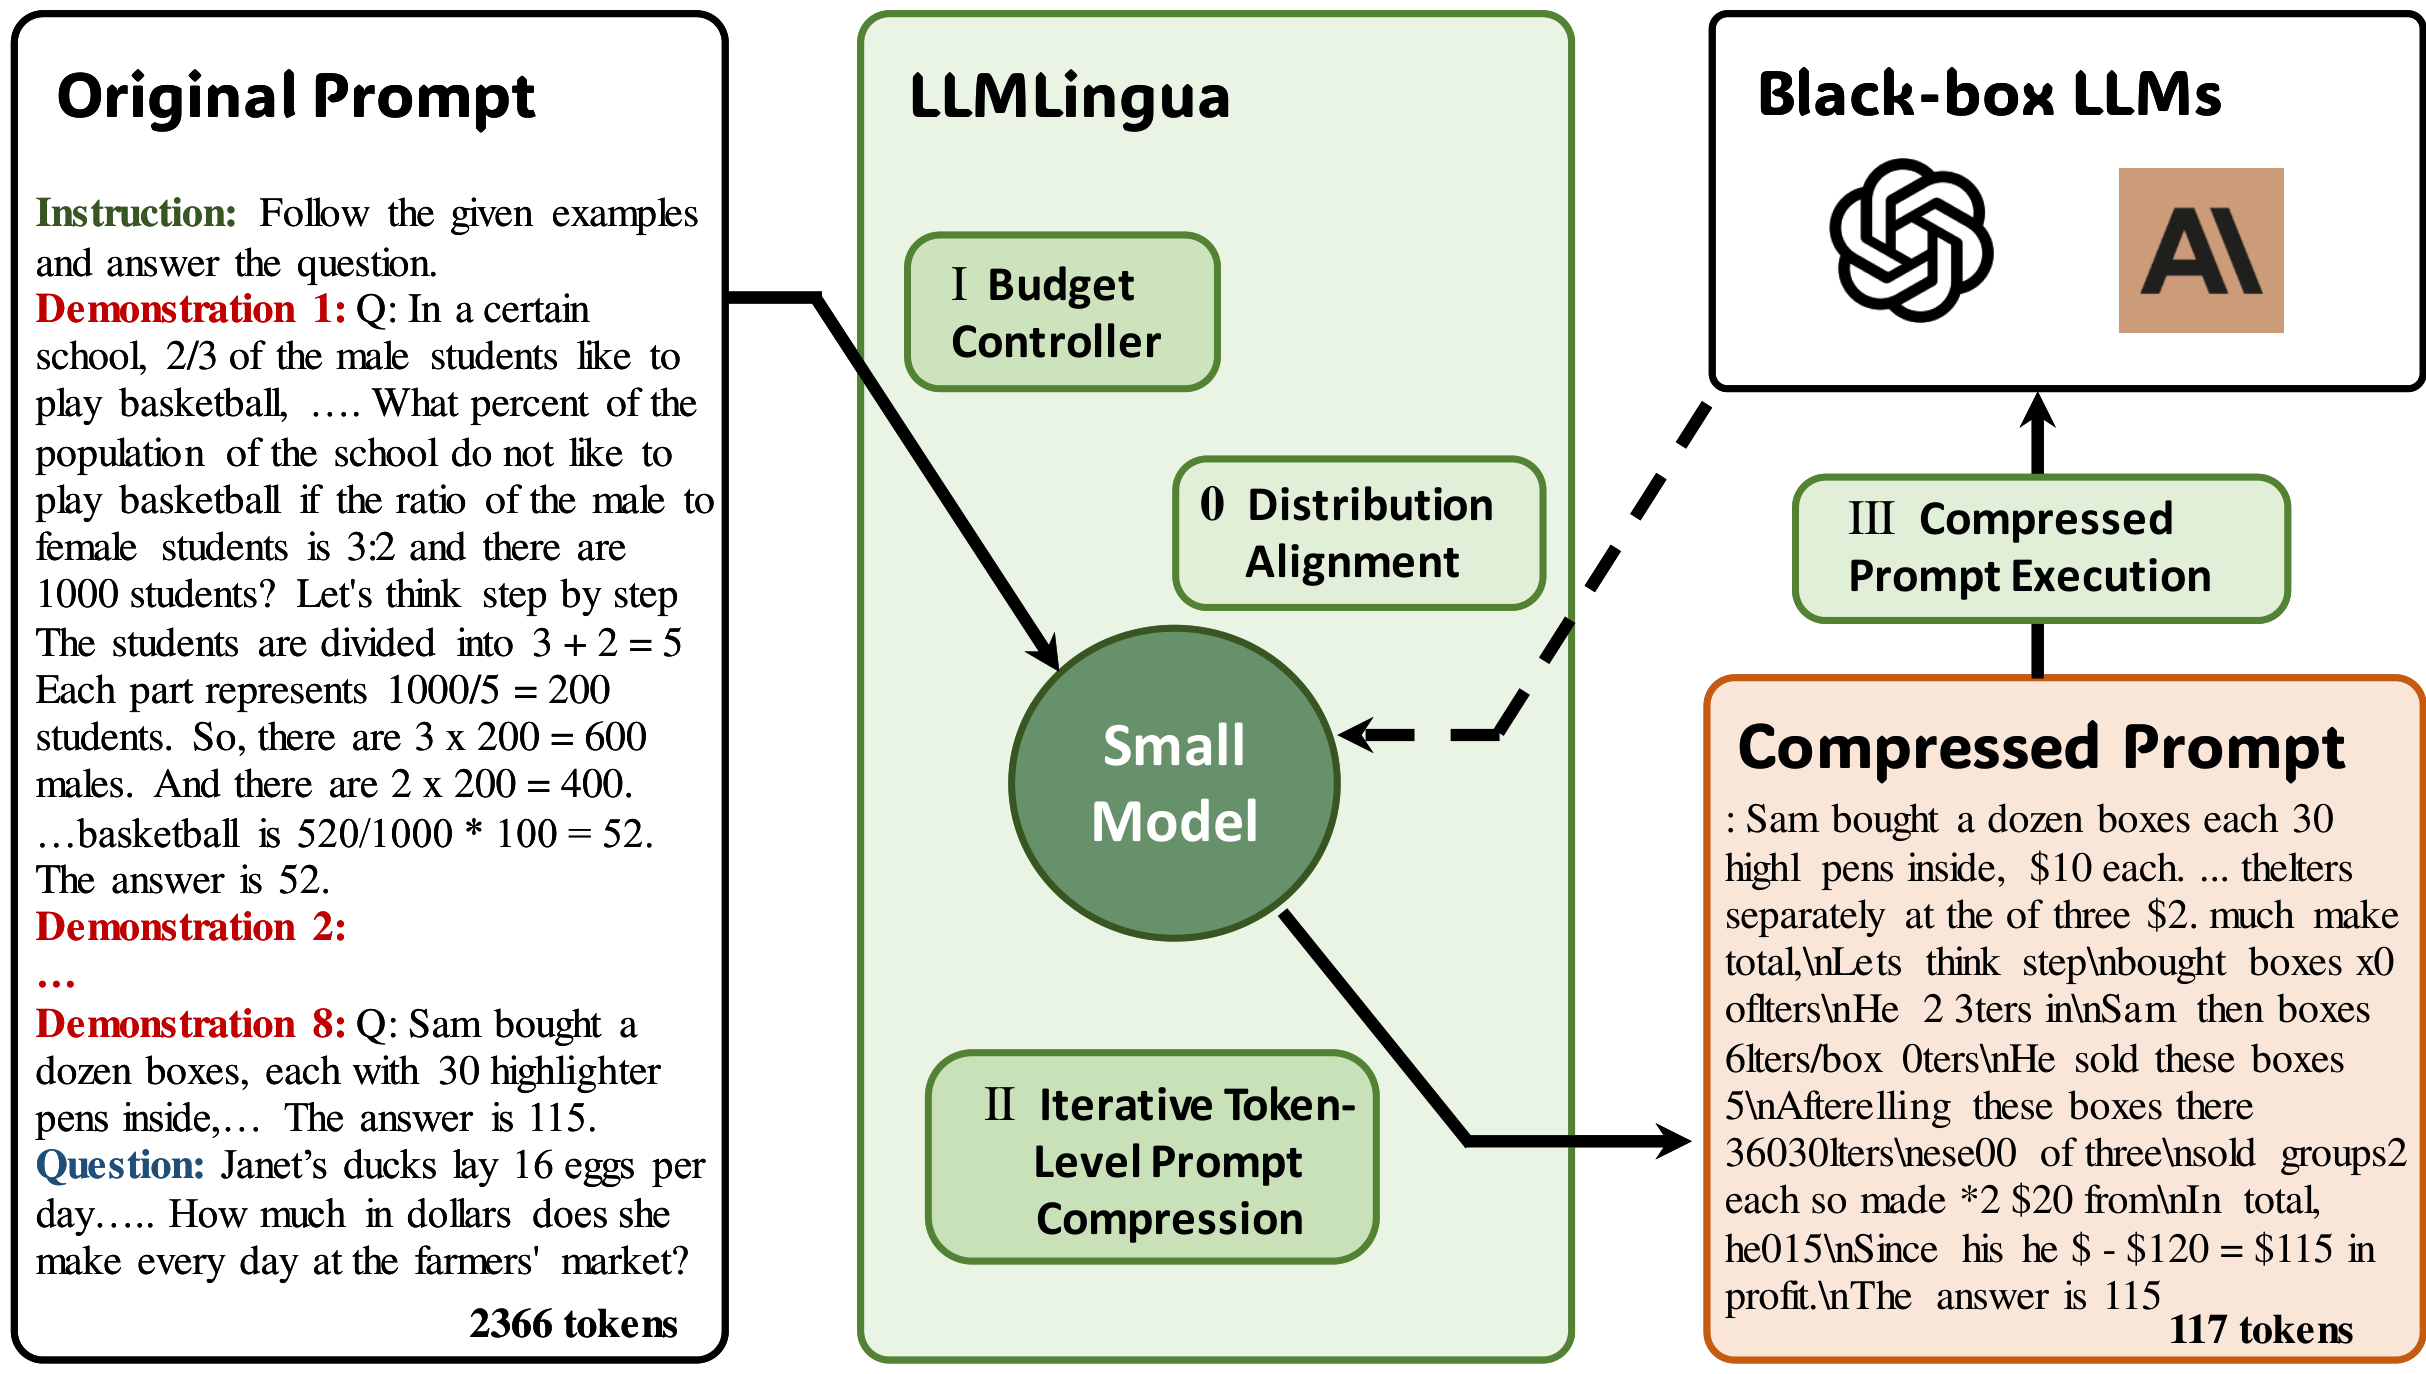
\includegraphics[width=\linewidth,height=0.5\textheight,keepaspectratio]{images/long-context/llmlingua_fig1_framework.png}\\[0.2em]
      {\scriptsize GSM8K on GPT-3.5-Turbo: the 2,366-token chain-of-thought prompt shrinks to 117 tokens ($20\times$) while exact match moves from 78.85 to 77.33. Selective Context reaches 44.20 at $15\times$.\par}
      \vspace{0.3em}
      {\scriptsize Jiang et al., ``LLMLingua: Compressing Prompts for Accelerated Inference of Large Language Models,'' EMNLP 2023, \href{https://arxiv.org/abs/2310.05736v2}{arXiv:2310.05736v2}, Figure~1; numbers from Table~2. Selective Context: Li et al., ``Compressing Context to Enhance Inference Efficiency of Large Language Models,'' EMNLP 2023, \href{https://arxiv.org/abs/2310.06201v1}{arXiv:2310.06201v1}.\par}
  \end{columns}
\end{frame}

\begin{frame}{Question-Aware Compression: LongLLMLingua}
  \begin{columns}[T,onlytextwidth]
    \column{0.46\textwidth}
      \begin{itemize}\scriptsize\itemsep0.35em
        \item[\textcolor{red}{$\blacktriangleright$}] Question-agnostic deletion keeps whatever is surprising, relevant or not. On NaturalQuestions with 20 retrieved documents at $4\times$, LLMLingua scores 23.5 with the answer in document 10, below the 56.1 of GPT-3.5-Turbo given no documents.
        \item[\textcolor{red}{$\blacktriangleright$}] \textbf{Coarse step:} rank documents by the perplexity of the question given each document, with ``We can get the answer to this question in the given documents'' appended to the question. Lowest perplexity ranks first.
        \item[\textcolor{red}{$\blacktriangleright$}] \textbf{Fine step:} score each token by its \textbf{contrastive perplexity}
          \[ c_i = \mathrm{ppl}(x_i \mid x_{<i}) - \mathrm{ppl}(x_i \mid x^{\mathrm{q}}, x_{<i}), \]
          where $x^{\mathrm{q}}$ is the question and $\mathrm{ppl}$ the small LM's perplexity of token $x_i$. Tokens that the question makes predictable score high.
        \item[\textcolor{red}{$\blacktriangleright$}] \textbf{Reordering} puts the top-ranked documents first, against the position bias, and top-ranked documents keep more tokens. \textbf{Subsequence recovery} swaps entity fragments the LLM copies into its answer for the full span in the original prompt.
      \end{itemize}
    \column{0.52\textwidth}
      \centering
      \vspace{0.4em}
      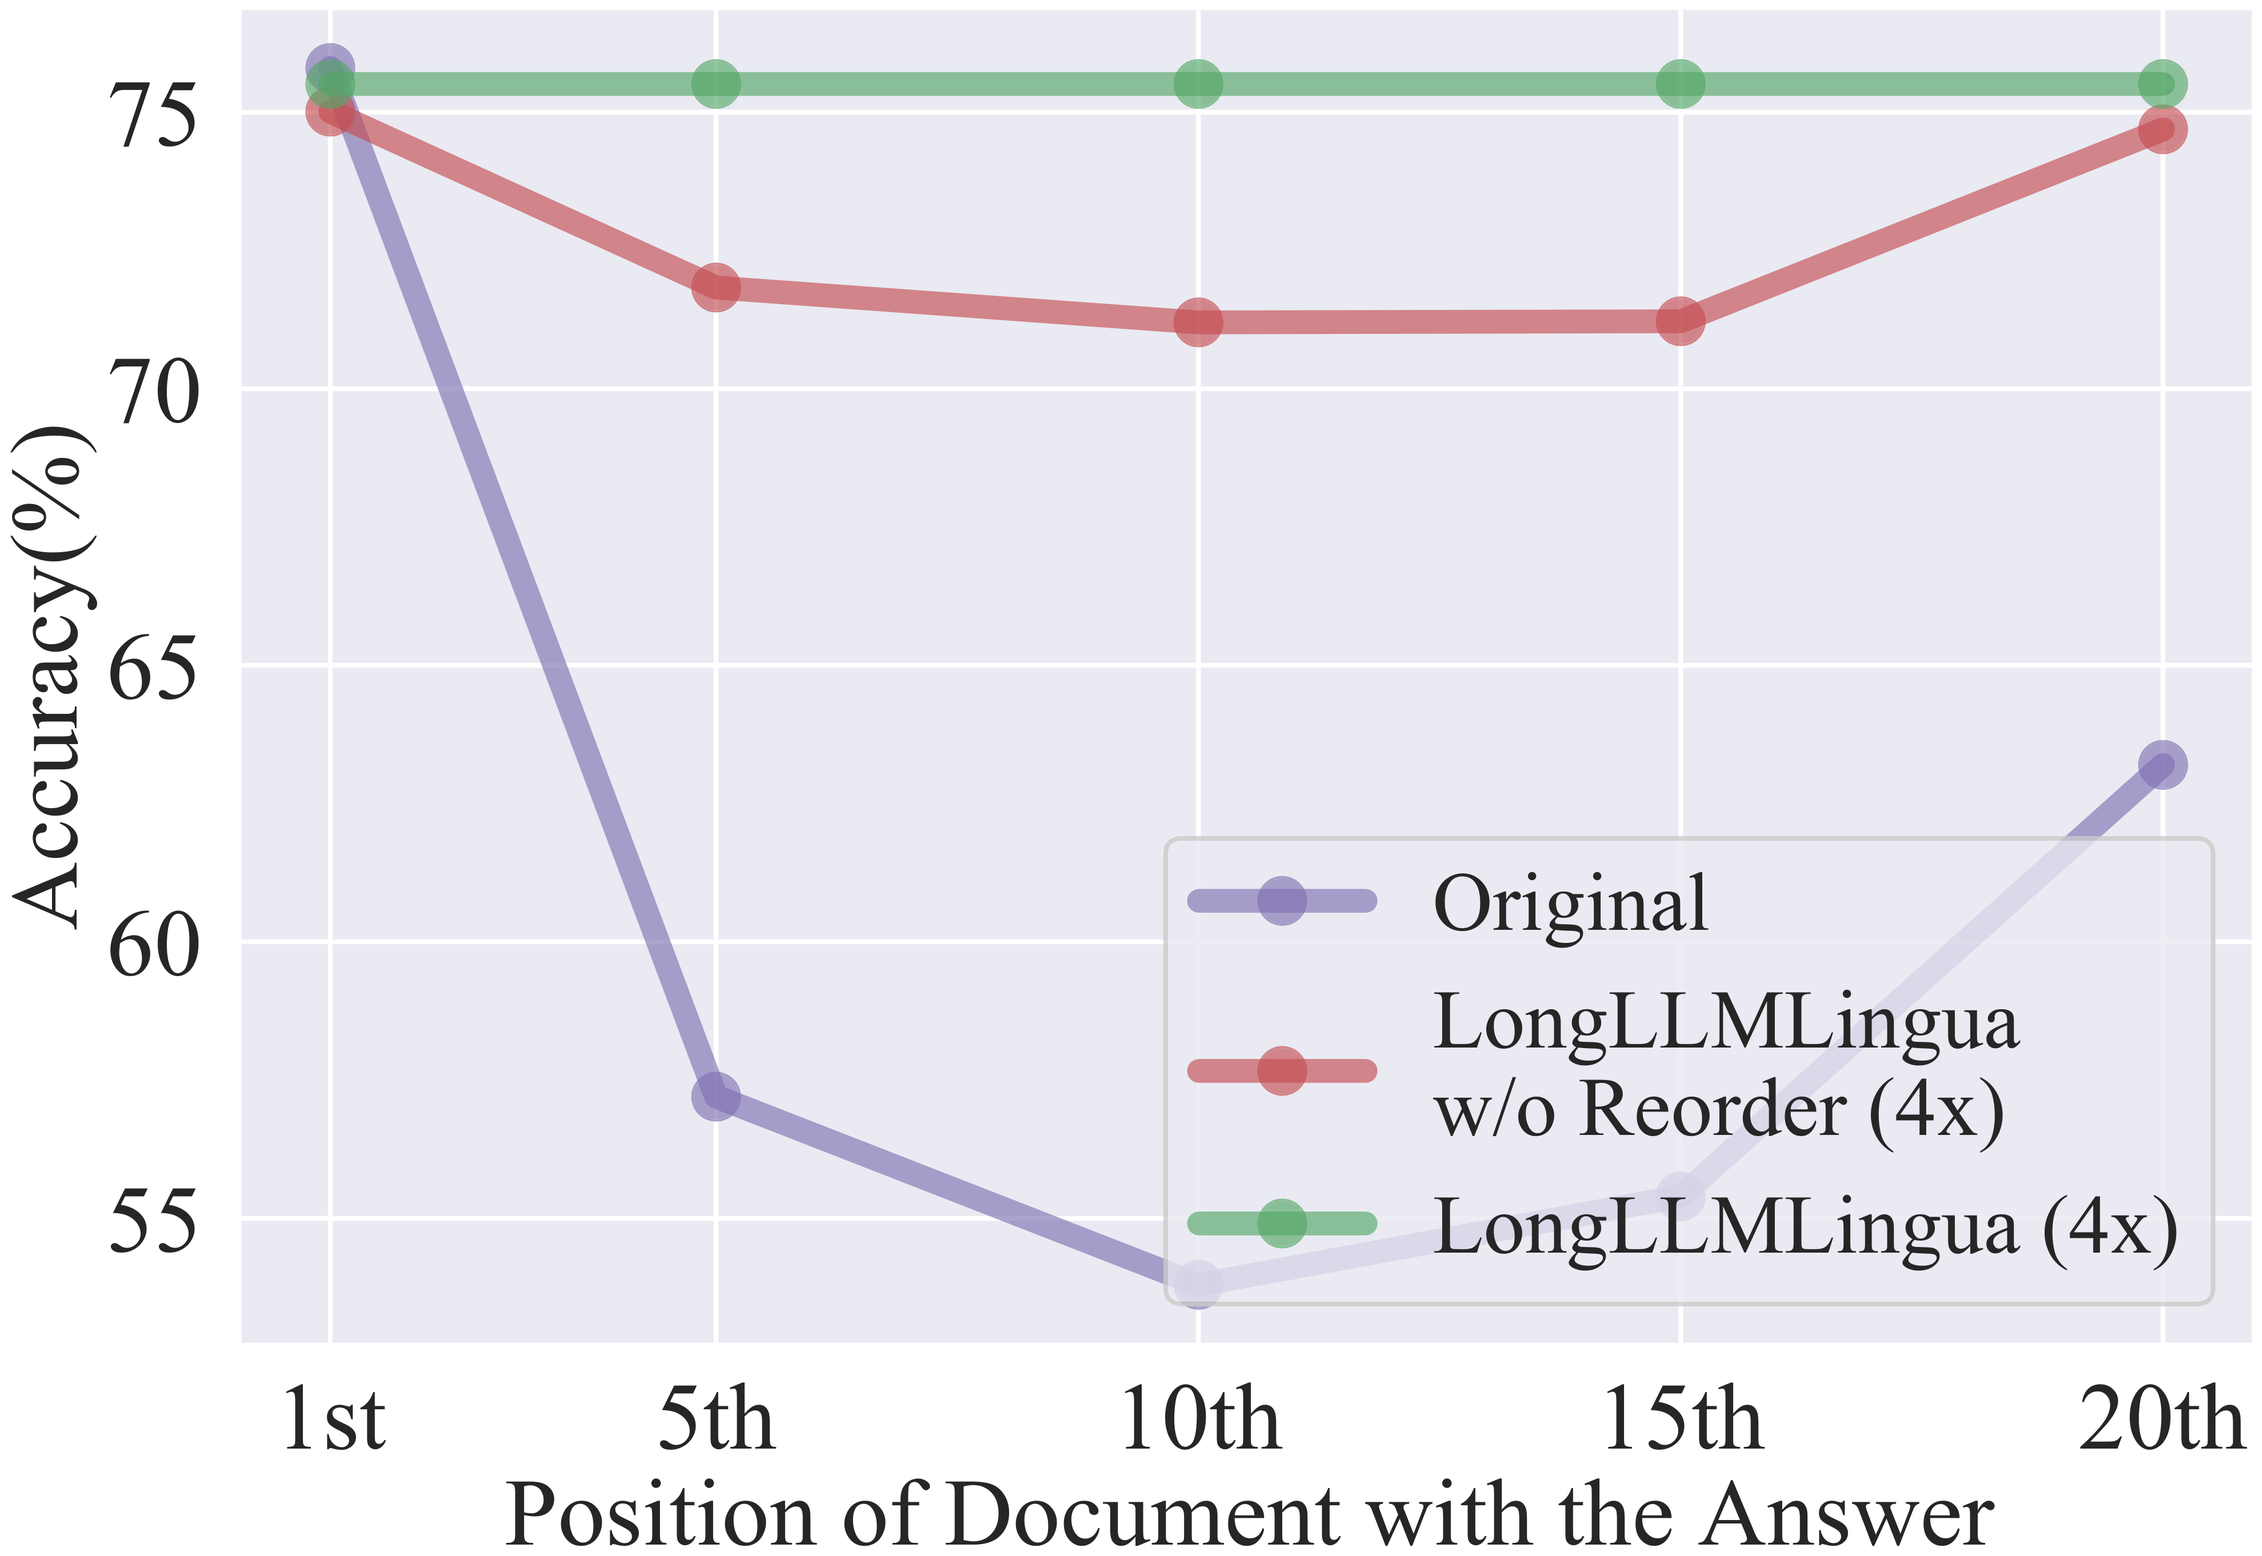
\includegraphics[width=\linewidth,height=0.5\textheight,keepaspectratio]{images/long-context/longllmlingua_fig1b_answer_position.png}\\[0.2em]
      {\scriptsize Accuracy against the position of the answer document among 20 (GPT-3.5-Turbo, NaturalQuestions). With the answer in document 10: 54.1 on the full 2,946-token prompt, 71.2 at 748 tokens ($3.9\times$), 75.5 with reordering, at half the end-to-end latency.\par}
      \vspace{0.3em}
      {\scriptsize Jiang et al., ``LongLLMLingua: Accelerating and Enhancing LLMs in Long Context Scenarios via Prompt Compression,'' ACL 2024, \href{https://arxiv.org/abs/2310.06839v2}{arXiv:2310.06839v2}, Figure~1(b); numbers from Table~1.\par}
  \end{columns}
\end{frame}

\begin{frame}{LLMLingua-2: Deletion as Token Classification}
  \begin{columns}[T,onlytextwidth]
    \column{0.46\textwidth}
      \begin{itemize}\scriptsize\itemsep0.35em
        \item[\textcolor{red}{$\blacktriangleright$}] Self-information from a causal LM is a proxy: it sees only the left context, and nothing trains it to compress.
        \item[\textcolor{red}{$\blacktriangleright$}] \textbf{Data distillation:} GPT-4 compresses MeetingBank meeting transcripts in chunks of at most 512 tokens under strict rules: remove words only, keep their order, add nothing. As in knowledge distillation, a large model's outputs become the training labels of a small one.
        \item[\textcolor{red}{$\blacktriangleright$}] \textbf{Labels:} each original word is marked keep or drop by fuzzy matching against GPT-4's output, which tolerates changes of tense or plural. Samples with the 5\% highest variation rate (words GPT-4 invented) or the 10\% largest alignment gap are discarded.
        \item[\textcolor{red}{$\blacktriangleright$}] \textbf{Compressor:} a bidirectional encoder (XLM-RoBERTa-large, or multilingual BERT for the small version) with a linear keep/drop head, trained with cross-entropy. For a budget of $\tilde n$ words it keeps the $\tilde n$ words with the highest keep probability, in their original order.
        \item[\textcolor{red}{$\blacktriangleright$}] Trained on meetings only, it beats LLMLingua on LongBench, a suite of long-input tasks, under a 2,000-token budget (average 39.1 against 34.6) but trails the question-aware LongLLMLingua (48.0).
      \end{itemize}
    \column{0.52\textwidth}
      {\scriptsize The same GSM8K demonstration under both compressors (start shown):\par}
      \vspace{0.1em}
      \begin{tcolorbox}[colframe=gray!60, colback=gray!6, boxrule=0.4pt, left=3pt, right=3pt, top=2pt, bottom=2pt]
        \scriptsize\textbf{Original, 249 tokens:} Sam bought a dozen boxes, each with 30 highlighter pens inside, for \$10 each box. He rearranged five of these boxes\ldots\\[0.1em]
        \textbf{LLMLingua, 144} (117 in LLMLingua's Figure~1): Sam bought a dozen boxes each 30 highl pens inside, \$10 each. He reanged five of boxes\ldots\\[0.1em]
        \textbf{LLMLingua-2, 138:} Sam bought dozen 30 highlighter pens \$10 rearranged five boxes into six highlighters\ldots
      \end{tcolorbox}
      \vspace{0.2em}
      {\scriptsize Seconds on one V100 GPU (MeetingBank); rows 1--3 time the compressor alone. Uncompressed end to end: 14.9.\par}
      \vspace{0.1em}
      {\centering\scriptsize\setlength{\tabcolsep}{4pt}
      \begin{tabular}{lccc}
        \toprule
        \textbf{Compression ratio} & $2\times$ & $3\times$ & $5\times$ \\
        \midrule
        Selective Context & 15.9 & 15.6 & 15.5 \\
        LLMLingua & 2.9 & 2.1 & 1.5 \\
        LLMLingua-2 & 0.5 & 0.4 & 0.4 \\
        \addlinespace[0.2em]
        End to end, LLMLingua-2 & 9.4 & 7.5 & 5.2 \\
        \bottomrule
      \end{tabular}\par}
      \vspace{0.3em}
      {\scriptsize Pan et al., ``LLMLingua-2: Data Distillation for Efficient and Faithful Task-Agnostic Prompt Compression,'' Findings of ACL 2024, \href{https://arxiv.org/abs/2403.12968v2}{arXiv:2403.12968v2}; Figure~12, Tables~2 and 5.\par}
  \end{columns}
\end{frame}

\begin{frame}{Gist Tokens: Learning to Compress the Prompt}
  \begin{columns}[T,onlytextwidth]
    \column{0.46\textwidth}
      \begin{itemize}\scriptsize\itemsep0.35em
        \item[\textcolor{red}{$\blacktriangleright$}] \textbf{Gisting} inserts $M$ copies of a new token \texttt{<G>} between the instruction and the input, and changes the attention mask so that tokens after the gist tokens cannot attend to anything before them. The instruction then reaches the output only through the gist tokens' activations, and ordinary instruction fine-tuning with this mask teaches the model to compress, at no extra training cost.
        \item[\textcolor{red}{$\blacktriangleright$}] The keys and values over the gist tokens act like soft prompts, but the model produces them from the prompt itself, in one forward pass and with no training per task. They are cached and reused for every input.
        \item[\textcolor{red}{$\blacktriangleright$}] LLaMA-7B and FLAN-T5-XXL with one gist token: human-written instructions of about 26 tokens become one ($26\times$). Judged by ChatGPT against the same model trained without the gist mask, the win rates are 45.8\% and 42.5\% (ties count half; 50\% is parity).
        \item[\textcolor{red}{$\blacktriangleright$}] Against encoding the full prompt, a cached gist saves 40\% of FLOPs and 4--7\% of wall time. Against caching the full prompt's keys and values it saves little compute, but $26\times$ more prompts fit in the same memory.
      \end{itemize}
    \column{0.52\textwidth}
      \centering
      \vspace{0.4em}
      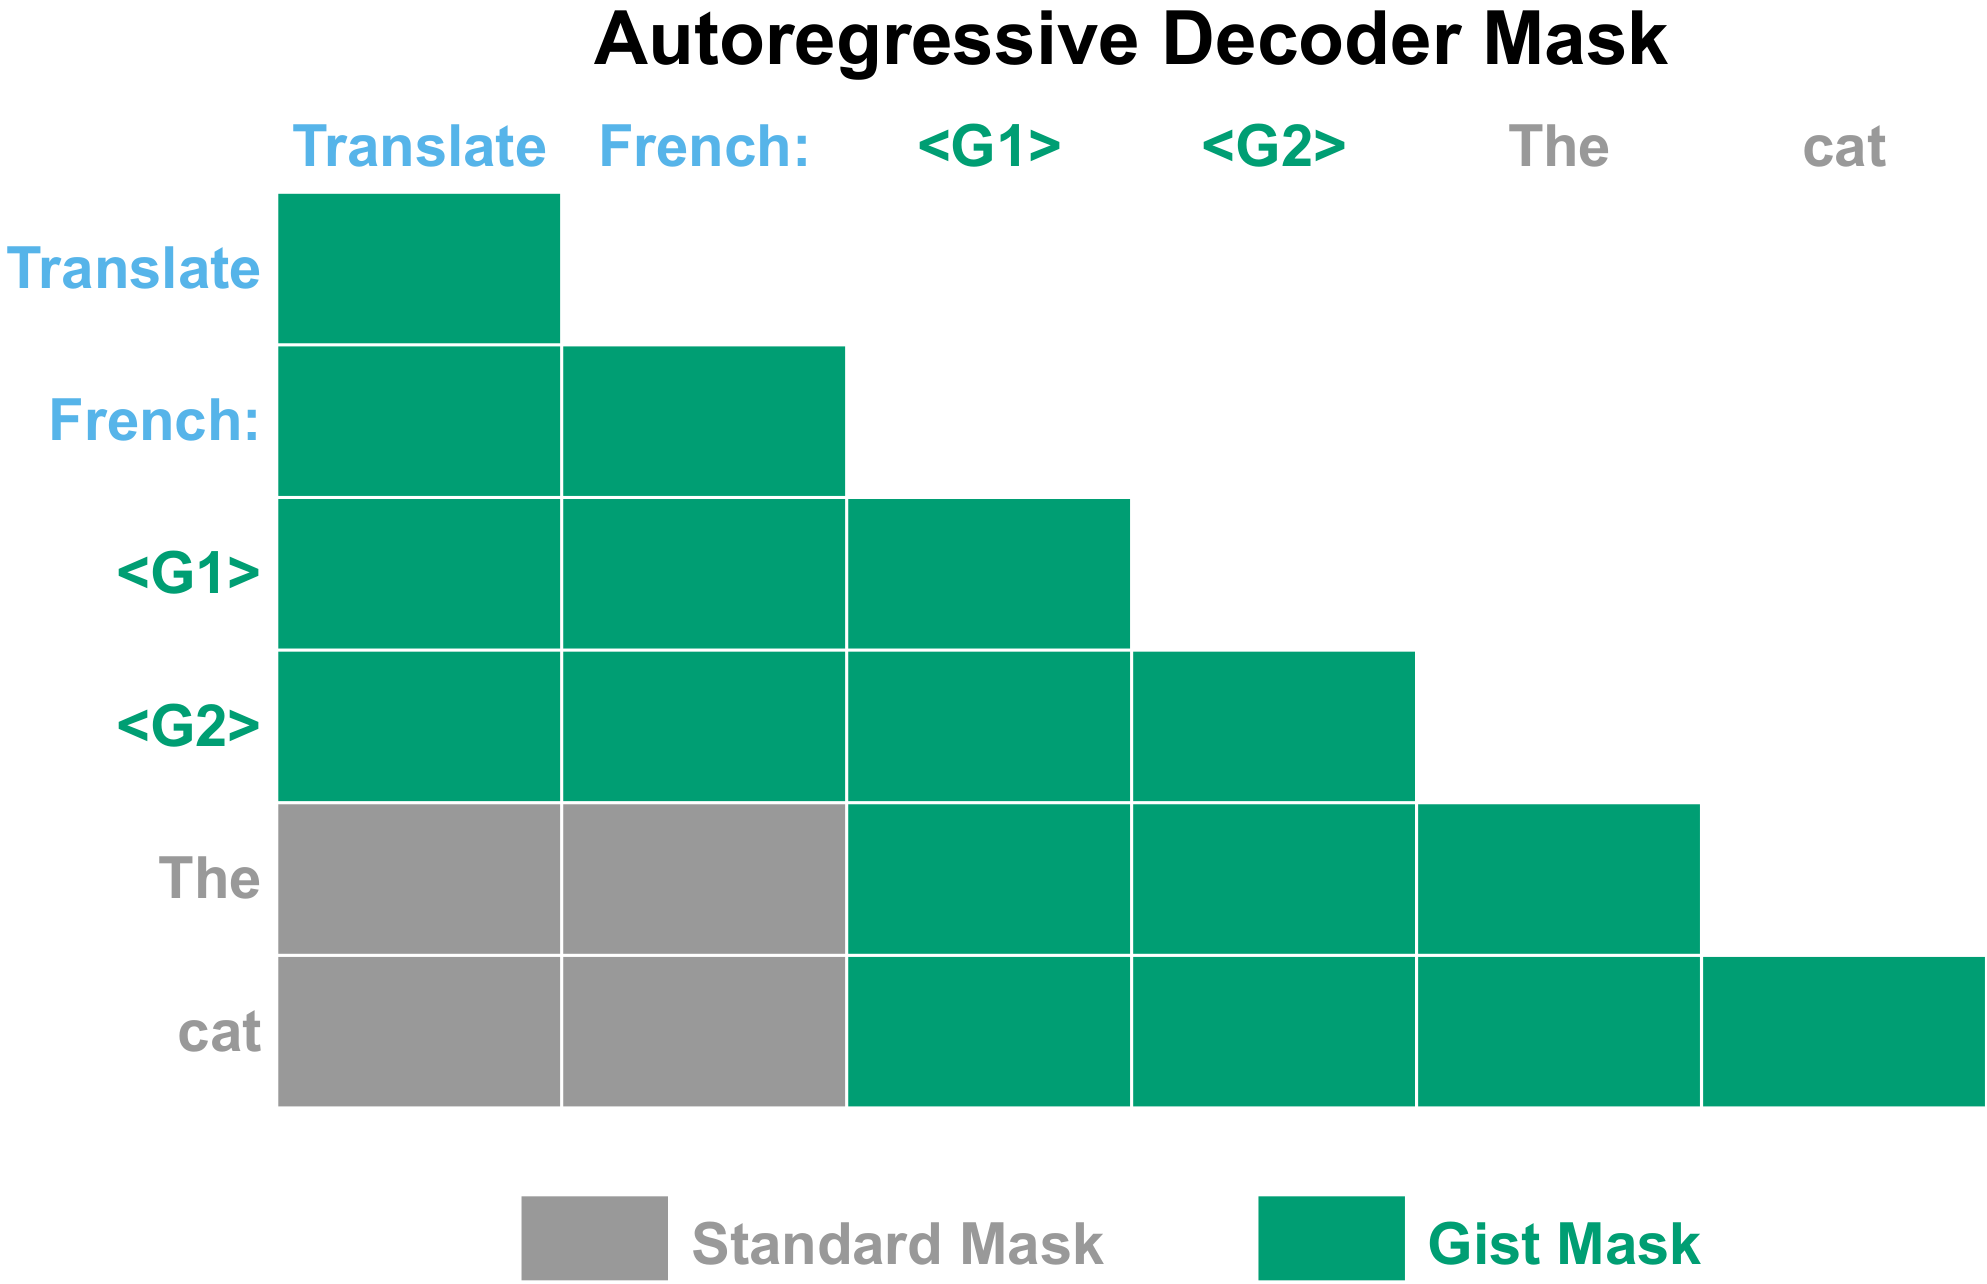
\includegraphics[width=\linewidth,height=0.52\textheight,keepaspectratio]{images/long-context/gist_fig2a_decoder_mask.png}\\[0.2em]
      {\scriptsize Row tokens attend to column tokens. Grey cells are visible under the ordinary causal mask and hidden under the gist mask, so ``The cat'' sees the instruction only through \texttt{<G1>} and \texttt{<G2>}.\par}
      \vspace{0.3em}
      {\scriptsize Mu et al., ``Learning to Compress Prompts with Gist Tokens,'' NeurIPS 2023, \href{https://arxiv.org/abs/2304.08467v3}{arXiv:2304.08467v3}, Figure~2(a); numbers from Tables~1 and 3.\par}
  \end{columns}
\end{frame}

\begin{frame}{In-Context Autoencoder (ICAE)}
  \begin{columns}[T,onlytextwidth]
    \column{0.46\textwidth}
      \begin{itemize}\scriptsize\itemsep0.35em
        \item[\textcolor{red}{$\blacktriangleright$}] \textbf{Encoder:} the LLM with a LoRA adapter reads the context followed by $M$ learned memory tokens; its outputs at those positions are the $M$ \textbf{memory slots}. \textbf{Decoder:} the same LLM, frozen, reads the slots in place of the context. About 1\% extra parameters are trained.
        \item[\textcolor{red}{$\blacktriangleright$}] \textbf{Pretraining} on the Pile uses two self-supervised losses: autoencoding (after a special \texttt{[AE]} token, reproduce the context from the slots) and text continuation. \textbf{Fine-tuning} then uses PwC, 240k (context, prompt, response) triples: Pile texts with prompts and responses written by GPT-4.
        \item[\textcolor{red}{$\blacktriangleright$}] Default: 512 tokens into $M = 128$ slots ($4\times$). Ordinary text comes back almost exactly (BLEU 99.3) but random token strings do not (BLEU 0.2), so the slots hold what the LLM can rebuild from its own knowledge.
        \item[\textcolor{red}{$\blacktriangleright$}] Llama-2-7B-chat answering from 128 slots, judged by GPT-4: against the full context, 19.6\% wins, 45.4\% losses, 35.0\% ties; against a 128-token summary written by GPT-4, 34.1\% wins and 17.6\% losses.
        \item[\textcolor{red}{$\blacktriangleright$}] For a batch of 8 inputs of 2,048 tokens, compressing and then decoding is $3.3\times$ faster than decoding from the full context.
      \end{itemize}
    \column{0.52\textwidth}
      \centering
      \vspace{0.6em}
      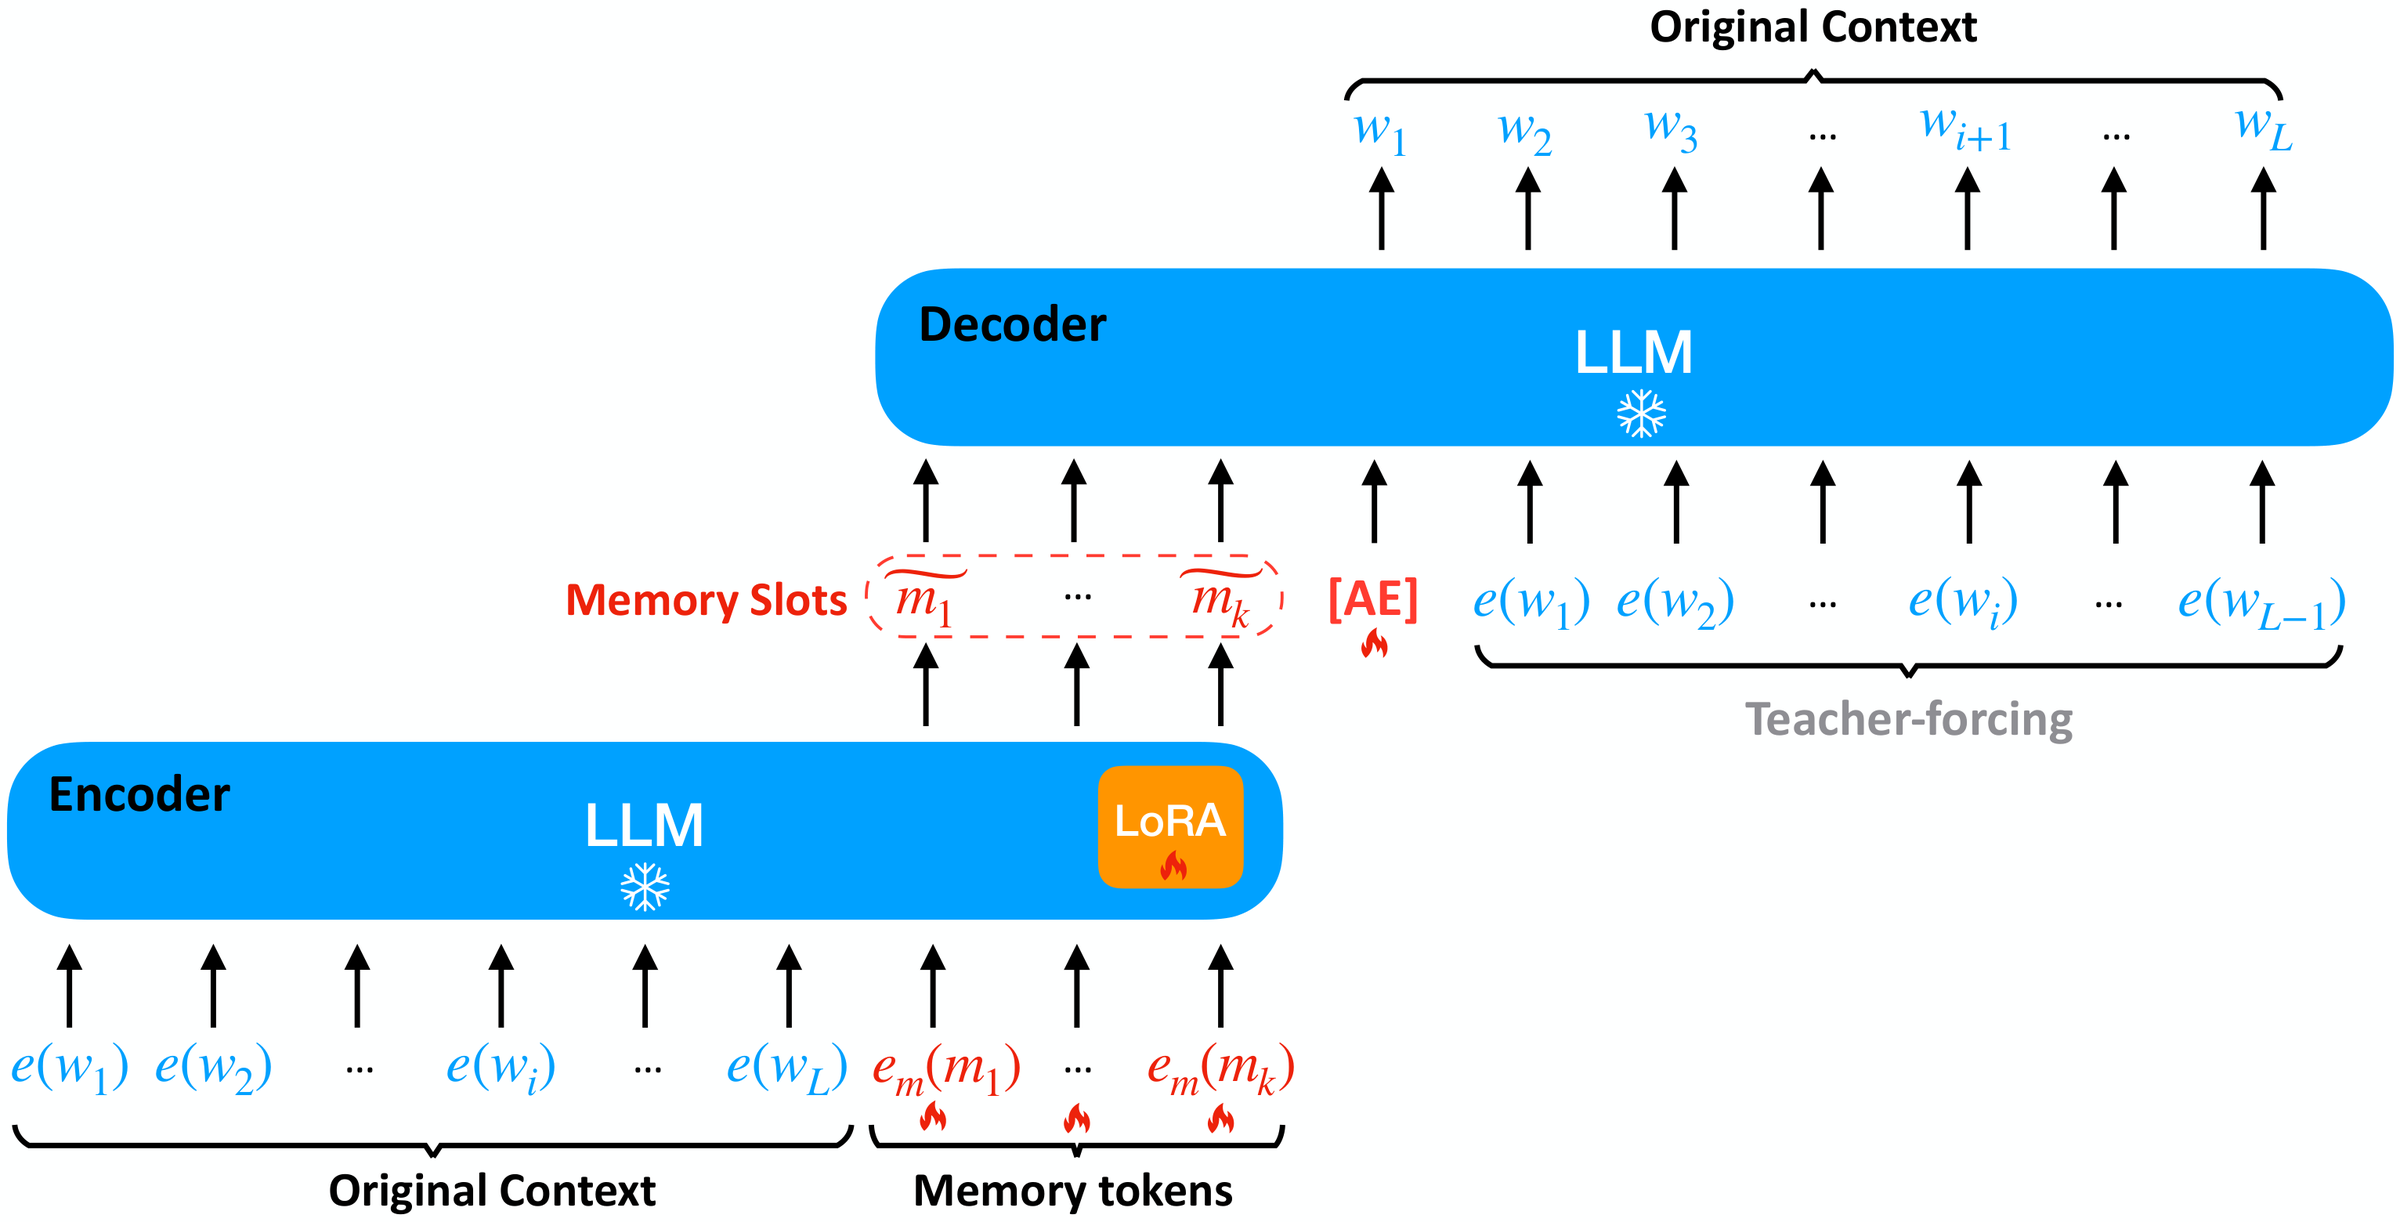
\includegraphics[width=\linewidth,height=0.5\textheight,keepaspectratio]{images/long-context/icae_fig3_architecture.png}\\[0.2em]
      {\scriptsize Autoencoding pretraining: the frozen decoder rebuilds the context $w_1,\dots,w_L$ from the memory slots. The figure's $k$ is $M$ here, and its $L$ counts context tokens.\par}
      \vspace{0.3em}
      {\scriptsize Ge et al., ``In-context Autoencoder for Context Compression in a Large Language Model,'' ICLR 2024, \href{https://arxiv.org/abs/2307.06945v4}{arXiv:2307.06945v4}, Figure~3; numbers from Tables~3, 4, 5 and 7.\par}
  \end{columns}
\end{frame}

\begin{frame}{AutoCompressors: Compressing Recursively}
  \begin{columns}[T,onlytextwidth]
    \column{0.46\textwidth}
      \begin{itemize}\scriptsize\itemsep0.35em
        \item[\textcolor{red}{$\blacktriangleright$}] Split a long document into segments of $s$ tokens and append 50 summary tokens to each segment. Their output states are the segment's \textbf{summary vectors}, a soft prompt for the text that follows.
        \item[\textcolor{red}{$\blacktriangleright$}] \textbf{Summary accumulation:} segment $i$ is read with the summary vectors of all earlier segments prepended, so each new summary is computed from fresh text plus the older summaries.
        \item[\textcolor{red}{$\blacktriangleright$}] Training needs no labels. The loss is ordinary next-token prediction over the whole document, so a summary is good exactly when it helps predict later text. Segment lengths are randomised, and gradients stop after two segments to save memory.
        \item[\textcolor{red}{$\blacktriangleright$}] OPT-2.7B with $s = 2{,}048$ stores 40 tokens per summary vector. Fine-tuned on 30,720-token sequences, its perplexity on the last segment still falls as the compressed context grows from 14,336 to 28,672 tokens (11.21 to 11.18).
        \item[\textcolor{red}{$\blacktriangleright$}] Llama-2-7B: 4,096 tokens in 100 vectors predict about as well as 512 plain tokens (perplexity 5.08 against 5.06). Full attention over all 4,096 plain tokens is still better (4.80).
        \item[\textcolor{red}{$\blacktriangleright$}] Carrying a compressed state from one segment to the next is the recurrent-memory pattern.
      \end{itemize}
    \column{0.52\textwidth}
      \centering
      \vspace{0.4em}
      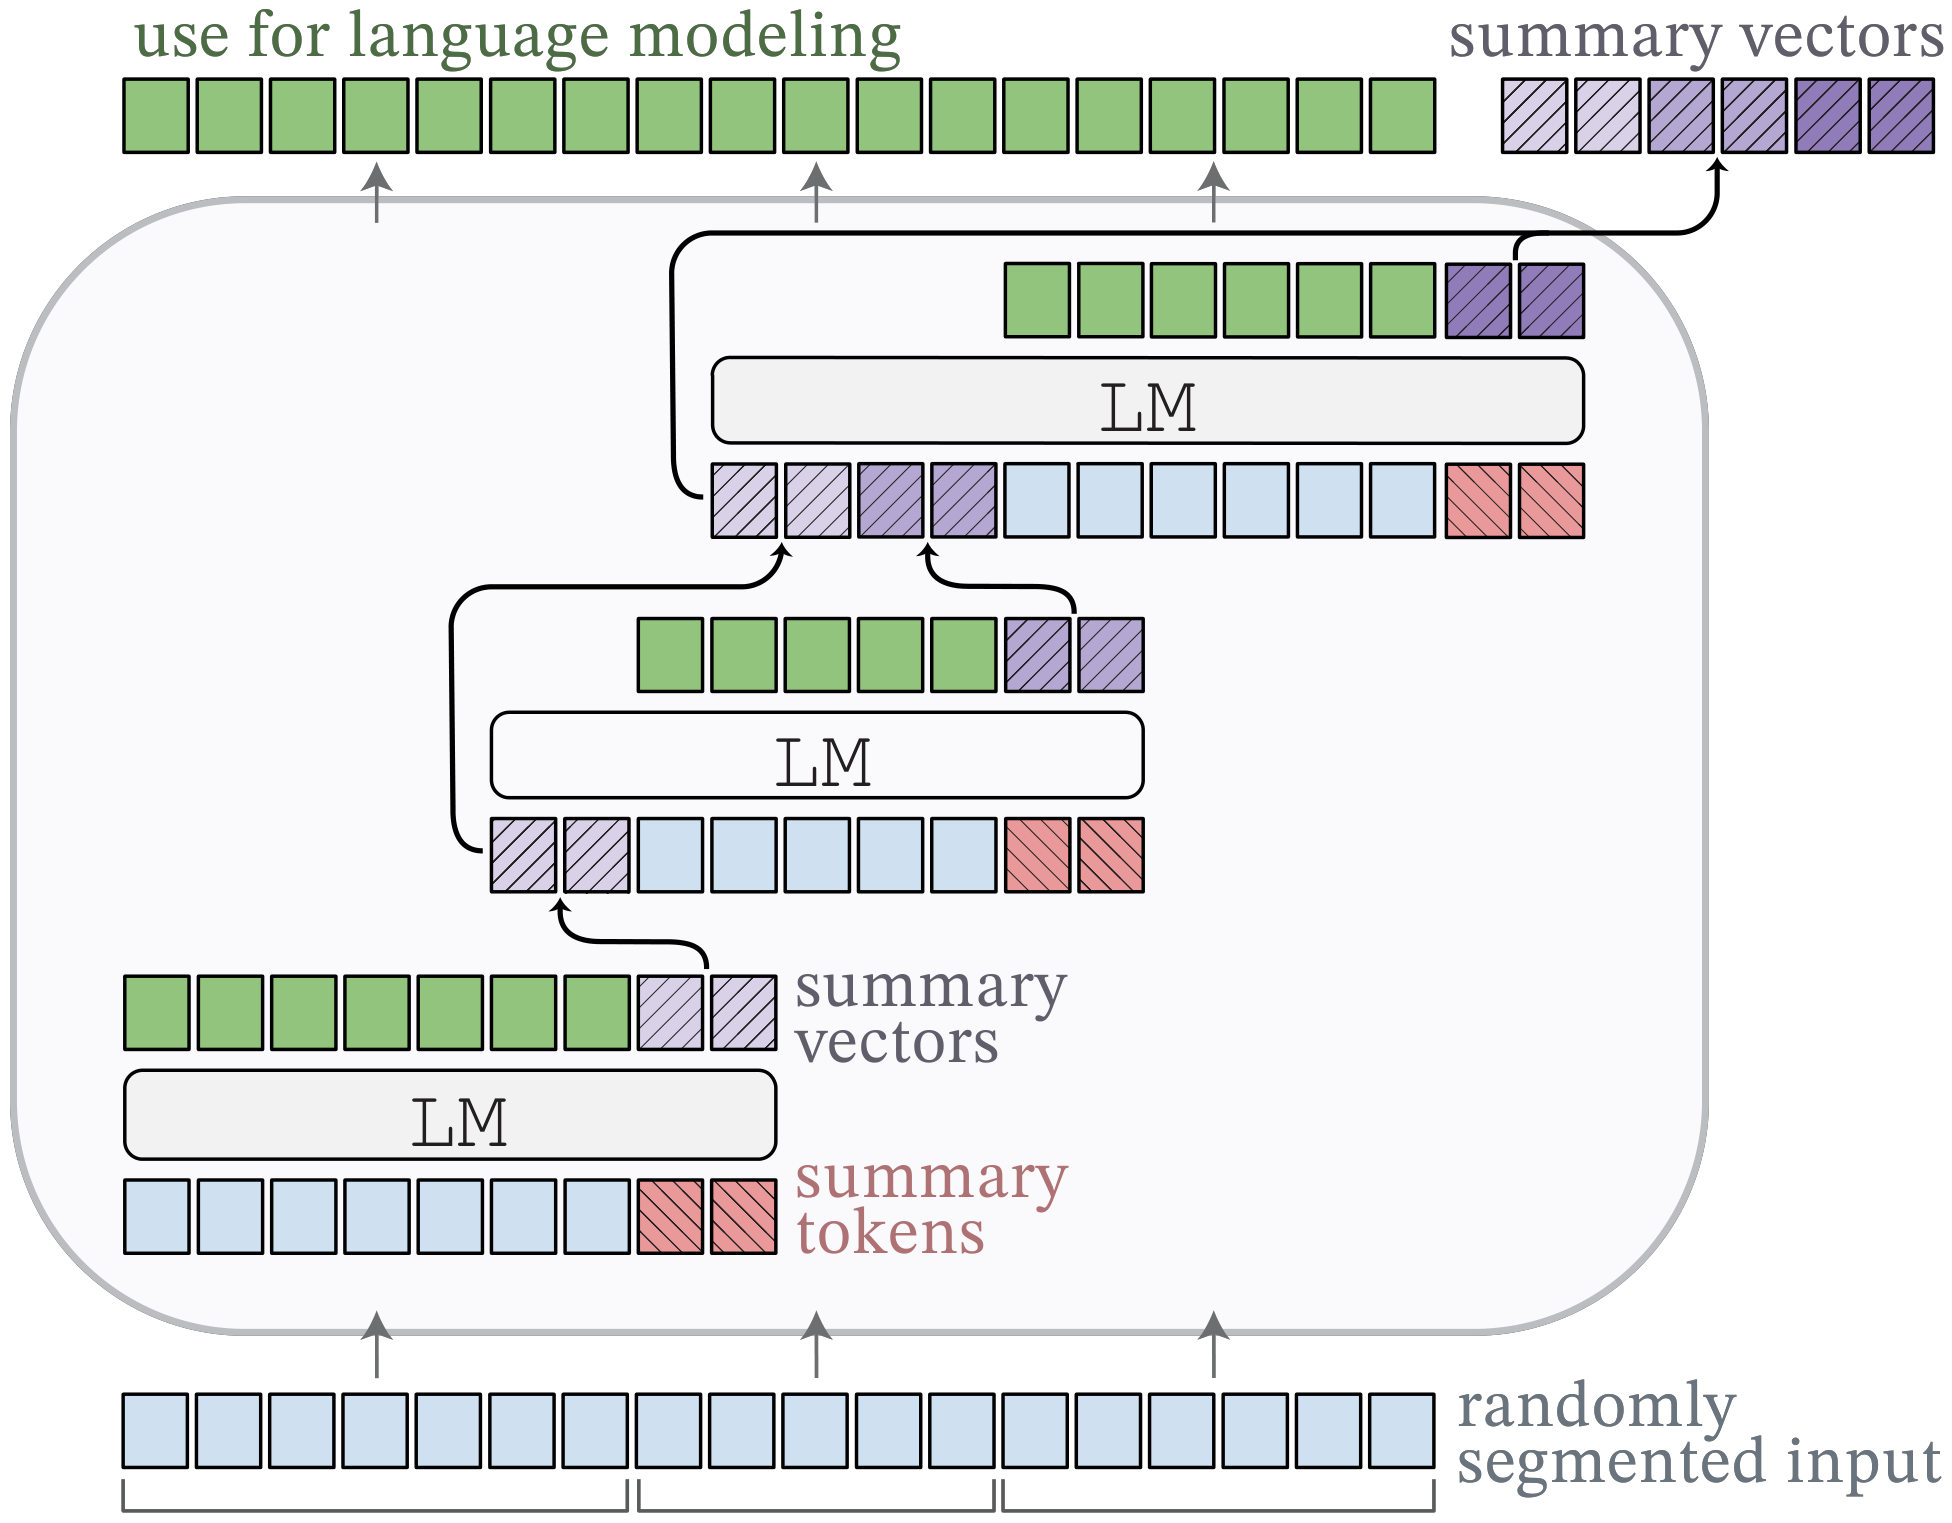
\includegraphics[width=\linewidth,height=0.62\textheight,keepaspectratio]{images/long-context/autocompressors_fig1_summary_accumulation.png}\\[0.2em]
      {\scriptsize Chevalier et al., ``Adapting Language Models to Compress Contexts,'' EMNLP 2023, \href{https://arxiv.org/abs/2305.14788v2}{arXiv:2305.14788v2}, Figure~1; numbers from Tables~2 and 3.\par}
  \end{columns}
\end{frame}

\begin{frame}{What Compression Costs}
  \centering
  {\scriptsize\setlength{\tabcolsep}{4pt}
  \begin{tabular}{p{2.3cm} p{1.0cm} p{2.0cm} p{1.25cm} p{1.75cm} p{3.6cm}}
    \toprule
    \textbf{Method} & \textbf{Output} & \textbf{Needs} & \textbf{Question} & \textbf{Reported ratio} & \textbf{Reported effect} \\
    \midrule
    Selective Context & text & small LM & agnostic & about $2\times$ & BERTScore $-0.023$ \\
    LLMLingua & text & small LM & agnostic & up to $20\times$ & GSM8K 78.85 to 77.33 \\
    LongLLMLingua & text & small LM & aware & about $4\times$ & NaturalQuestions 54.1 to 71.2 \\
    LLMLingua-2 & text & small encoder & agnostic & $2$--$5\times$ & end to end $1.6$--$2.9\times$ faster \\
    \addlinespace[0.2em]
    Gist tokens & vectors & fine-tuned LLM & agnostic & $26\times$ & 40\% fewer FLOPs \\
    ICAE & vectors & LoRA encoder & agnostic & $4\times$ & $3.3\times$ faster \\
    AutoCompressors & vectors & fine-tuned LLM & agnostic & about $40\times$ & 4,096 tokens $\approx$ 512 plain \\
    \bottomrule
  \end{tabular}\par}
  \vspace{0.3em}
  \raggedright
  % parskip's paragraph gap applies between full-width list items; the frame group keeps this local
  \setlength{\parskip}{0.2em}
  \begin{itemize}\scriptsize\itemsep0.1em
    \item[\textcolor{red}{$\blacktriangleright$}] \textbf{Exact strings go first.} LLMLingua's $20\times$ GSM8K prompt reads ``highl pens'' and ``36030lters'', LongLLMLingua needs subsequence recovery to restore names, a gist model returned ``Culture'' for ``Arts \& Culture'', and ICAE rebuilds random token strings at BLEU 0.2. Spans that must survive verbatim, such as code, identifiers and numbers, are safer left uncompressed.
    \item[\textcolor{red}{$\blacktriangleright$}] \textbf{Hard or soft.} Hard output is readable, works with any API and needs no change to the target model; the reported operating points are about $20\times$ on redundant few-shot prompts and $2$--$5\times$ on documents. Soft output packs more into each position (ICAE's 128 slots beat a 128-token GPT-4 summary), but it is tied to one model's weights, costs a training run and cannot be read.
    \item[\textcolor{red}{$\blacktriangleright$}] \textbf{Aware or agnostic.} Seeing the question lifted accuracy at $4\times$ from 23.5 to 71.2 on the same test (answer in document 10), but the compressed prompt must then be rebuilt for every question. Query-agnostic output is computed once and cached.
  \end{itemize}
  {\scriptsize Each ratio is the paper's own operating point on its own benchmark, so the rows are not directly comparable. Sources as on the previous slides.\par}
\end{frame}
